\chapter{Дарақтағы алгоритмдер}

\index{дарақ}

Дарақ -- өзара байланысты, циклі жоқ граф. Дарақ $n$ 
төбеден және $n-1$ қырдан тұрады. Кез келген қырды 
алып тастаса,  дарақ екі компонентке бөлінеді және 
кез келген жерге қыр қосса, дарақта цикл пайда болады. 
Оған қоса, дарақта әр екі төбенің арасында жалғыз жол болады.

Мысалы, төмендегі дарақ 8 төбеден және 7 қырдан тұрады:
\begin{center}
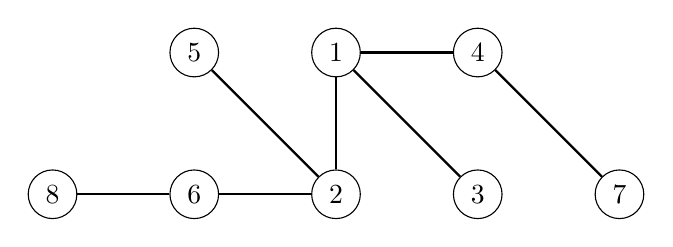
\begin{tikzpicture}[scale=0.9]
\node[draw, circle] (1) at (0,3) {$1$};
\node[draw, circle] (2) at (2,3) {$4$};
\node[draw, circle] (3) at (0,1) {$2$};
\node[draw, circle] (4) at (2,1) {$3$};
\node[draw, circle] (5) at (4,1) {$7$};
\node[draw, circle] (6) at (-2,3) {$5$};
\node[draw, circle] (7) at (-2,1) {$6$};
\node[draw, circle] (8) at (-4,1) {$8$};
\path[draw,thick,-] (1) -- (2);
\path[draw,thick,-] (1) -- (3);
\path[draw,thick,-] (1) -- (4);
\path[draw,thick,-] (2) -- (5);
\path[draw,thick,-] (3) -- (6);
\path[draw,thick,-] (3) -- (7);
\path[draw,thick,-] (7) -- (8);
\end{tikzpicture}
\end{center}

\index{жапырақ}

Дарақтың жапырақтары -- дәрежесі 1-ге тең (яғни
жалғыз бір көршісі бар) төбелер.
Мысалы, жоғарыда берілген дарақтың жапырақтары --
$3$, $5$, $7$ және $8$-төбелер.

\index{түбір}
\index{түбірлі дарақ}

Түбірлі дарақта бір төбе дарақтың 
түбірі ретінде таңдалады, ал басқа 
төбелер оның астында орналасады.
Үлгідегі графтың түбірі -- $1$-төбе:

\begin{center}
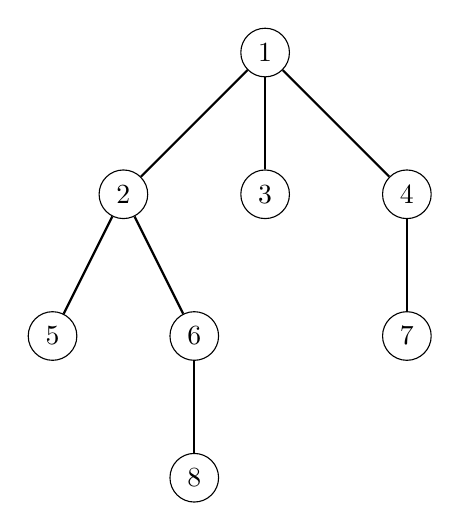
\begin{tikzpicture}[scale=0.9]
\node[draw, circle] (1) at (0,3) {$1$};
\node[draw, circle] (4) at (2,1) {$4$};
\node[draw, circle] (2) at (-2,1) {$2$};
\node[draw, circle] (3) at (0,1) {$3$};
\node[draw, circle] (7) at (2,-1) {$7$};
\node[draw, circle] (5) at (-3,-1) {$5$};
\node[draw, circle] (6) at (-1,-1) {$6$};
\node[draw, circle] (8) at (-1,-3) {$8$};
\path[draw,thick,-] (1) -- (2);
\path[draw,thick,-] (1) -- (3);
\path[draw,thick,-] (1) -- (4);
\path[draw,thick,-] (2) -- (5);
\path[draw,thick,-] (2) -- (6);
\path[draw,thick,-] (4) -- (7);
\path[draw,thick,-] (6) -- (8);
\end{tikzpicture}
\end{center}

\index{ұл}
\index{әке}

Түбірлі дарақтағы төбенің ұлдары -- 
төмендегі көршілері, ал төбенің әкесі --
үстіндегі көршісі. Түбірден басқа, 
әр төбенің бір әкесі болады. Мысалы 
үлгідегі дарақта $2$-төбенің ұлдары -- $5$
және $6$-төбелер, ал оның әкесі $1$-төбе саналады.

\index{ішдарақ}

Төбенің ішдарағы деп дарақтың сол төбеден және оның барша ұрпақтарынан тұратын бөлігін атаймыз. Басқаша айтқанда, $v$ төбесінің ішдарағы $u$ төбесінің $u$-дан дарақтың түбіріне дейінгі жолында міндетті түрде $v$ кездесетін төбелерінен тұрады.

Мысалға, жоғарыдағы дарақта $2$-төбенің ішдарағы $2$,
$5$, $6$ және $8$ төбелерден тұрады.

\begin{center}
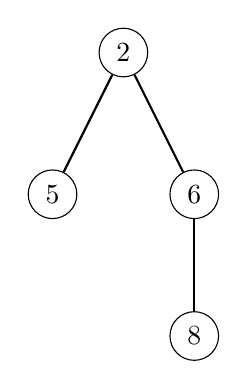
\begin{tikzpicture}[scale=0.9]
\node[draw, circle] (2) at (-2,1) {$2$};
\node[draw, circle] (5) at (-3,-1) {$5$};
\node[draw, circle] (6) at (-1,-1) {$6$};
\node[draw, circle] (8) at (-1,-3) {$8$};
\path[draw,thick,-] (2) -- (5);
\path[draw,thick,-] (2) -- (6);
\path[draw,thick,-] (6) -- (8);
\end{tikzpicture}
\end{center}

\section{Дарақты аралап шығу}

Жалпы графты аралайтын алгоритмдерді 
дарақты аралау үшін де қолдануға болады.
Бірақ дарақты аралайтын кодты жазу оңайырақ.
Себебі дарақта циклдер болмайды және төбеге
бірнеше бағыттан келу мүмкін емес.

Дарақты өтіп шығу үшін әдетте кез келген төбеден 
тереңдігі бойынша ізденіс жүргізіледі. Мысалы, төмендегі
рекурсивті функцияны қолдануға болады:

\begin{lstlisting}
void dfs(int s, int e) {
    // process node s
    for (auto u : adj[s]) {
        if (u != e) dfs(u, s);
    }
}
\end{lstlisting}

Әлі бармаған төбелерді ажырату мақсатында қазіргі төбе $s$ параметрінің қасына ертерек өтіп кеткен төбе $e$ параметрін қосуымызға болады. 

Келесі функцияның шақыруы ізденісті $x$ төбесінен
бастайды:

\begin{lstlisting}
dfs(x, 0);
\end{lstlisting}

Бірінші шақырғанда $e=0$. Өйткені бұл
жерде ешқандай алдыңғы төбе жоқ және дарақтың
кез келген бағытына өтуге рұқсат етіледі.

\subsubsection{Динамикалық бағдарламалау}

Дарақты аралау барысында динамикалық бағдарламалауды ақпараттарды есептеу
үшін қолдана аламыз. Мысалы, оның көмегімен
түбірлі дарақта $O(n)$ уақытта әр 
төбенің ішдарағындағы төбелердің
санын немесе төбеден жапыраққа дейінгі ең 
ұзын жолдың ұзындығын есептеуге болады.

Үлгі ретінде келесі есепті қарастырамыз. Мысалы әр $s$ төбесі үшін $\texttt{count}[s]$
мәнін сақтаймыз. Бұл мән бізге $s$ төбесінің ішдарағындағы төбелер санын көрсетеді. Ішдарақ
төбенің өзін және оның ұлдарының ішдарағындағы барлық төбелерді қамтиды. Осылайша біз төбелердің санын
берілген код арқылы есептей аламыз:

\begin{lstlisting}
void dfs(int s, int e) {
    count[s] = 1;
    for (auto u : adj[s]) {
        if (u == e) continue;
        dfs(u, s);
        count[s] += count[u];
    }
}
\end{lstlisting}

\section{Диаметр}

\index{диаметр}

Дарақтың \key{диаметрі} -- дарақтағы екі 
төбенің арасындағы жолдың максималды 
ұзындығы.
Мысалы, келесі дарақты қарастырайық:
\begin{center}
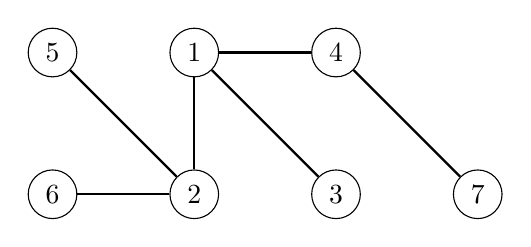
\begin{tikzpicture}[scale=0.9]
\node[draw, circle] (1) at (0,3) {$1$};
\node[draw, circle] (2) at (2,3) {$4$};
\node[draw, circle] (3) at (0,1) {$2$};
\node[draw, circle] (4) at (2,1) {$3$};
\node[draw, circle] (5) at (4,1) {$7$};
\node[draw, circle] (6) at (-2,3) {$5$};
\node[draw, circle] (7) at (-2,1) {$6$};
\path[draw,thick,-] (1) -- (2);
\path[draw,thick,-] (1) -- (3);
\path[draw,thick,-] (1) -- (4);
\path[draw,thick,-] (2) -- (5);
\path[draw,thick,-] (3) -- (6);
\path[draw,thick,-] (3) -- (7);
\end{tikzpicture}
\end{center}
Дарақтың диаметрі 4-ке тең,
ол келесі жолға сәйкес келеді:
\begin{center}
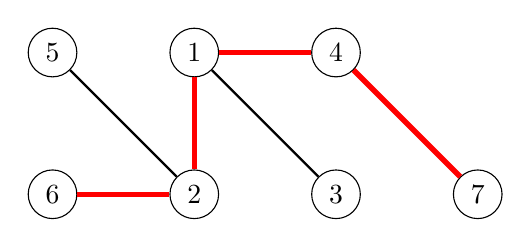
\begin{tikzpicture}[scale=0.9]
\node[draw, circle] (1) at (0,3) {$1$};
\node[draw, circle] (2) at (2,3) {$4$};
\node[draw, circle] (3) at (0,1) {$2$};
\node[draw, circle] (4) at (2,1) {$3$};
\node[draw, circle] (5) at (4,1) {$7$};
\node[draw, circle] (6) at (-2,3) {$5$};
\node[draw, circle] (7) at (-2,1) {$6$};
\path[draw,thick,-] (1) -- (2);
\path[draw,thick,-] (1) -- (3);
\path[draw,thick,-] (1) -- (4);
\path[draw,thick,-] (2) -- (5);
\path[draw,thick,-] (3) -- (6);
\path[draw,thick,-] (3) -- (7);

\path[draw,thick,-,color=red,line width=2pt] (7) -- (3);
\path[draw,thick,-,color=red,line width=2pt] (3) -- (1);
\path[draw,thick,-,color=red,line width=2pt] (1) -- (2);
\path[draw,thick,-,color=red,line width=2pt] (2) -- (5);
\end{tikzpicture}
\end{center}
Ұзындықтары максималды бірнеше жол 
болуы мүмкін екенін ескерген дұрыс.
Жоғарыдағы жолда $6$-төбені $5$-төбемен
алмастырсақ, тағы бір ұзындығы 4-ке 
тең жолды табар едік.

Енді дарақтың диаметрін есептеу үшін уақытша күрделілігі
$O(n)$ болатын екі алгоритмді қарастырамыз.
Бірінші алгоритм динамикалық бағдарламалауға негізделген.
Ал екінші алгоритм тереңдігі бойынша екі ізденісті қолданады.

\subsubsection{1-алгоритм}

Көптеген дарақ есептерін шешуде мынадай жалпы тәсілді қолданамыз.
Алдымен дарақтағы кез келген бір төбені түбір етіп таңдап аламыз.
Кейін есепті әр ішдарақ үшін бөлек шығара береміз. 
Біздің диаметрді есептеу үшін қолданатын бірінші 
алгоритміміз де осындай идеяны ұстанады.

Мынадай маңызды ескертуді жадымызда сақтағанымыз жөн: Түбірлі дарақта әр
жолдың \emph{ең биік нүктесі} -- жолға жататын 
ең жоғарғы төбесі болады. Осылайша біз дарақтағы әр төбеге
ең биік нүктесі сол болатындай ұзындығы 
максималды жолды есептей аламыз. Осындай барлық
жолдардың біреуі дарақтың диаметріне тең болады.

Мысалы, төмендегі дарақта $1$-төбе 
диаметрдің бойында жататын ең жоғарғы төбе болып тұр:

\begin{center}
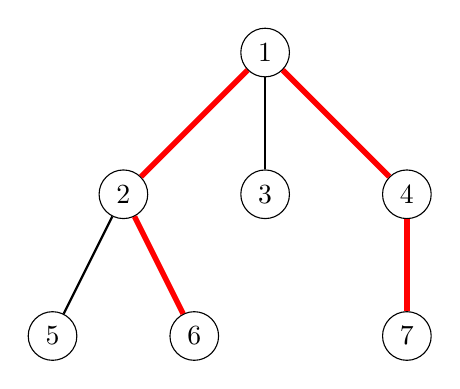
\begin{tikzpicture}[scale=0.9]
\node[draw, circle] (1) at (0,3) {$1$};
\node[draw, circle] (2) at (2,1) {$4$};
\node[draw, circle] (3) at (-2,1) {$2$};
\node[draw, circle] (4) at (0,1) {$3$};
\node[draw, circle] (5) at (2,-1) {$7$};
\node[draw, circle] (6) at (-3,-1) {$5$};
\node[draw, circle] (7) at (-1,-1) {$6$};
\path[draw,thick,-] (1) -- (2);
\path[draw,thick,-] (1) -- (3);
\path[draw,thick,-] (1) -- (4);
\path[draw,thick,-] (2) -- (5);
\path[draw,thick,-] (3) -- (6);
\path[draw,thick,-] (3) -- (7);

\path[draw,thick,-,color=red,line width=2pt] (7) -- (3);
\path[draw,thick,-,color=red,line width=2pt] (3) -- (1);
\path[draw,thick,-,color=red,line width=2pt] (1) -- (2);
\path[draw,thick,-,color=red,line width=2pt] (2) -- (5);
\end{tikzpicture}
\end{center}

Біз әр $x$-төбеде екі санды сақтаймыз:
\begin{itemize}
\item $\texttt{toLeaf}(x)$: $x$-тен бастап кез келген жапыраққа
дейінгі жолдың максималды ұзындығы
\item $\texttt{maxLength}(x)$: ең жоғарғы нүктесі $x$ болатын жолдың максималды ұзындығы.
\end{itemize}
Мысалы, жоғарыдағы дарақта
$1 \rightarrow 2 \rightarrow 6$ жолы болғандықтан
$\texttt{toLeaf}(1)=2$,
және $6 \rightarrow 2 \rightarrow 1 \rightarrow 4 \rightarrow 7$ 
жолы болғандықтан $\texttt{maxLength}(1)=4$.
Осы жағдайда диаметр -- $\texttt{maxLength}(1)$.

$O(n)$ уақыт ішінде барлық төбелер үшін осы мәндерді есептеуде динамикалық бағдарламалауды пайдалануға 
болады. Алдымен $\texttt{toLeaf}(x)$ мәнін 
есептеу үшін $x$ төбесінің ұлдарынан өтіп шығамыз. Олардың ішінен 
$\texttt{toLeaf}(c)$ максималды мәні бар
$c$ төбесін таңдап, бұл мәнге 1-ді қосамыз. Содан соң $\texttt{maxLength}(x)$ мәнін есептеу үшін
біз $\texttt{toLeaf}(a) + \texttt{toLeaf}(b)$ қосындысы максималды болатындай екі түрлі $a$ және $b$ ұл төбелерін таңдап, алынған мәнге 2-ні қосамыз. 

\subsubsection{2-алгоритм}

Дарақтың диаметрін есептеудің тағы бір тиімді әдісі
екі тереңдігі бойынша ізденіске негізделеді.
Алдымен біз дарақтағы 
кез келген бір $a$ төбесін таңдаймыз және 
тереңдігі бойынша ізденіс арқылы 
$a$ төбесінен ең алыс орналасқан $b$ төбесін табамыз.
Кейін біз екінші тереңдігі бойынша ізденіс арқылы
$b$ төбесінен ең алыс орналасқан $c$ төбесін табамыз.
Дарақтың диаметрі $b$ мен $c$ төбелерінің арақашықтығына
тең болады.

Келесі граф үшін $a$, $b$, $c$ төмендегідей нұсқада да кездесе алады:
\begin{center}
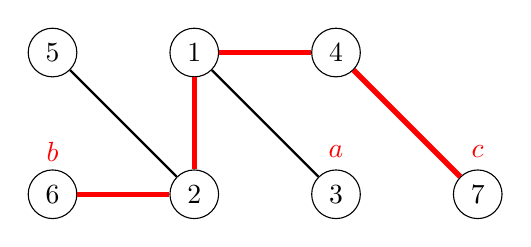
\begin{tikzpicture}[scale=0.9]
\node[draw, circle] (1) at (0,3) {$1$};
\node[draw, circle] (2) at (2,3) {$4$};
\node[draw, circle] (3) at (0,1) {$2$};
\node[draw, circle] (4) at (2,1) {$3$};
\node[draw, circle] (5) at (4,1) {$7$};
\node[draw, circle] (6) at (-2,3) {$5$};
\node[draw, circle] (7) at (-2,1) {$6$};
\path[draw,thick,-] (1) -- (2);
\path[draw,thick,-] (1) -- (3);
\path[draw,thick,-] (1) -- (4);
\path[draw,thick,-] (2) -- (5);
\path[draw,thick,-] (3) -- (6);
\path[draw,thick,-] (3) -- (7);
\node[color=red] at (2,1.6) {$a$};
\node[color=red] at (-2,1.6) {$b$};
\node[color=red] at (4,1.6) {$c$};

\path[draw,thick,-,color=red,line width=2pt] (7) -- (3);
\path[draw,thick,-,color=red,line width=2pt] (3) -- (1);
\path[draw,thick,-,color=red,line width=2pt] (1) -- (2);
\path[draw,thick,-,color=red,line width=2pt] (2) -- (5);
\end{tikzpicture}
\end{center}

"Бұл -- талғампаз әдіс, бірақ неге ол дұрыс жұмыс істейді?" - деген сұраққа жауап іздейміз. 

Ол дараққа басқаша қарауға көмектеседі. Оны көрсету үшін дарақтың 
диаметрін көлденең қойып, 
барлық басқа төбелер соған ілінетін түрін қарастырайық:
\begin{center}
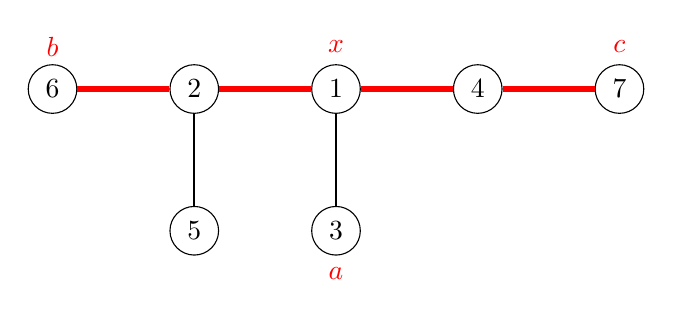
\begin{tikzpicture}[scale=0.9]
\node[draw, circle] (1) at (2,1) {$1$};
\node[draw, circle] (2) at (4,1) {$4$};
\node[draw, circle] (3) at (0,1) {$2$};
\node[draw, circle] (4) at (2,-1) {$3$};
\node[draw, circle] (5) at (6,1) {$7$};
\node[draw, circle] (6) at (0,-1) {$5$};
\node[draw, circle] (7) at (-2,1) {$6$};
\path[draw,thick,-] (1) -- (2);
\path[draw,thick,-] (1) -- (3);
\path[draw,thick,-] (1) -- (4);
\path[draw,thick,-] (2) -- (5);
\path[draw,thick,-] (3) -- (6);
\path[draw,thick,-] (3) -- (7);
\node[color=red] at (2,-1.6) {$a$};
\node[color=red] at (-2,1.6) {$b$};
\node[color=red] at (6,1.6) {$c$};
\node[color=red] at (2,1.6) {$x$};

\path[draw,thick,-,color=red,line width=2pt] (7) -- (3);
\path[draw,thick,-,color=red,line width=2pt] (3) -- (1);
\path[draw,thick,-,color=red,line width=2pt] (1) -- (2);
\path[draw,thick,-,color=red,line width=2pt] (2) -- (5);
\end{tikzpicture}
\end{center}

Мұнда $a$ төбесінің дарақтағы диаметрге қосылған
жері $x$ төбесімен белгіленген. $a$ төбесінен ең 
алыс орналасқан төбе -- $b$ төбесі, $c$ төбесі немесе 
$x$ төбесінен сондай немесе одан алыс арақашықтықта орналасқан қандай да бір басқа төбе.
Осылайша бұл төбе диаметрге сәйкес келетін жолдың 
шеткі төбесіне жарамды таңдау бола алады.
% Node $x$ indicates the place where the path
% from node $a$ joins the path that corresponds
% to the diameter.
% The farthest node from $a$
% is node $b$, node $c$ or some other node
% that is at least as far from node $x$.
% Thus, this node is always a valid choice for
% an endpoint of a path that corresponds to the diameter.

\section{Барлық ең ұзын жолдар}

Келесі қарастыратын есебіміз -- дарақтың әрбір
төбесінен басталатын ұзындығы максималды жолды
табу.
Бұл есеп дарақтың диаметрін табудың жалпылама
түріне ұқсас болғандықтан, оны $O(n)$ уақытта
шығара аламыз.

Мысалы, келесі дарақты қарастырайық:
\begin{center}
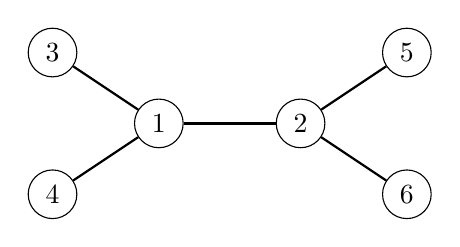
\begin{tikzpicture}[scale=0.9]
\node[draw, circle] (1) at (0,0) {$1$};
\node[draw, circle] (2) at (-1.5,-1) {$4$};
\node[draw, circle] (3) at (2,0) {$2$};
\node[draw, circle] (4) at (-1.5,1) {$3$};
\node[draw, circle] (6) at (3.5,-1) {$6$};
\node[draw, circle] (7) at (3.5,1) {$5$};
\path[draw,thick,-] (1) -- (2);
\path[draw,thick,-] (1) -- (3);
\path[draw,thick,-] (1) -- (4);
\path[draw,thick,-] (3) -- (6);
\path[draw,thick,-] (3) -- (7);
\end{tikzpicture}
\end{center}

Біз $\texttt{maxLength}(x)$ мәнінде $x$ төбесінен
басталатын дарақтағы максималды жолдың ұзындығын
сақтаймыз. Мысалы, жоғарыдағы дарақта $\texttt{maxLength}(4)=3$,
себебі, дарақта мынадай жол бар:
$4 \rightarrow 1 \rightarrow 2 \rightarrow 6$. Төменде
барлық төбелердің $\texttt{maxLength}$ мәндерін белгіледік:
\begin{center}
\begin{tabular}{l|lllllll}
$x$ төбесі  & 1 & 2 & 3 & 4 & 5 & 6 \\
$\texttt{maxLength}(x)$ & 2 & 2 & 3 & 3 & 3 & 3 \\
\end{tabular}
\end{center}


% denote the maximum length
% of a path that begins at node $x$.
% For example, in the above tree,
% $\texttt{maxLength}(4)=3$, because there
% is a path $4 \rightarrow 1 \rightarrow 2 \rightarrow 6$.
% Here is a complete table of the values:
% \begin{center}
% \begin{tabular}{l|lllllll}
% node $x$ & 1 & 2 & 3 & 4 & 5 & 6 \\
% $\texttt{maxLength}(x)$ & 2 & 2 & 3 & 3 & 3 & 3 \\
% \end{tabular}
% \end{center}

Бұл есепте де бастапқыда бір төбені түбір ретінде таңдаймыз:
% Also in this problem, a good starting point
% for solving the problem is to root the tree arbitrarily:
\begin{center}
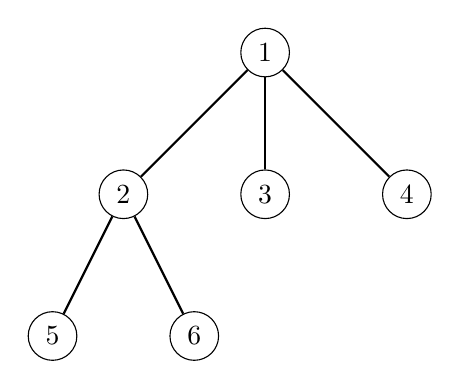
\begin{tikzpicture}[scale=0.9]
\node[draw, circle] (1) at (0,3) {$1$};
\node[draw, circle] (2) at (2,1) {$4$};
\node[draw, circle] (3) at (-2,1) {$2$};
\node[draw, circle] (4) at (0,1) {$3$};
\node[draw, circle] (6) at (-3,-1) {$5$};
\node[draw, circle] (7) at (-1,-1) {$6$};
\path[draw,thick,-] (1) -- (2);
\path[draw,thick,-] (1) -- (3);
\path[draw,thick,-] (1) -- (4);
\path[draw,thick,-] (3) -- (6);
\path[draw,thick,-] (3) -- (7);
\end{tikzpicture}
\end{center}

Есептің бірінші бөлігінде әр $x$ төбесі үшін
оның ұлы арқылы өтетін жолдың максималды ұзындығын
табу керек.
Мысалы, $1$-төбеден ең ұзын жол $2$-ұлынан
өтеді:
% The first part of the problem is to calculate for every node $x$
% the maximum length of a path that goes through a child of $x$.
% For example, the longest path from node 1
% goes through its child 2:
\begin{center}
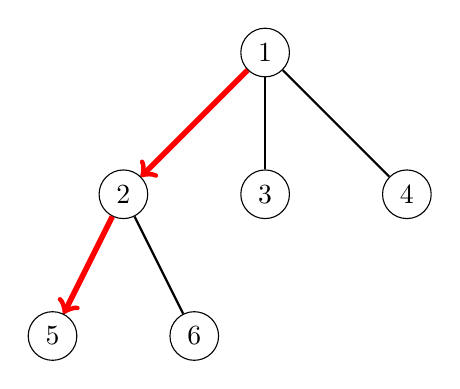
\begin{tikzpicture}[scale=0.9]
\node[draw, circle] (1) at (0,3) {$1$};
\node[draw, circle] (2) at (2,1) {$4$};
\node[draw, circle] (3) at (-2,1) {$2$};
\node[draw, circle] (4) at (0,1) {$3$};
\node[draw, circle] (6) at (-3,-1) {$5$};
\node[draw, circle] (7) at (-1,-1) {$6$};
\path[draw,thick,-] (1) -- (2);
\path[draw,thick,-] (1) -- (3);
\path[draw,thick,-] (1) -- (4);
\path[draw,thick,-] (3) -- (6);
\path[draw,thick,-] (3) -- (7);

\path[draw,thick,->,color=red,line width=2pt] (1) -- (3);
\path[draw,thick,->,color=red,line width=2pt] (3) -- (6);
\end{tikzpicture}
\end{center}
Бұл бөлікті $O(n)$ уақытта шығару оңай. Себебі алдында атап өткеніміздей
динамикалық бағдарламалау әдісін қолдана аламыз.
% This part is easy to solve in $O(n)$ time, because we can use
% dynamic programming as we have done previously.

Кейін есептің екінші бөлігінде әр $x$ төбесіне әкесі $p$ арқылы
жалғанатын максималды ұзын жолды есептеу керек.
Мысалы, $3$-төбеге $1$-төбеден келетін ең ұзын жол:
% Then, the second part of the problem is to calculate
% for every node $x$ the maximum length of a path
% through its parent $p$.
% For example, the longest path
% from node 3 goes through its parent 1:
\begin{center}
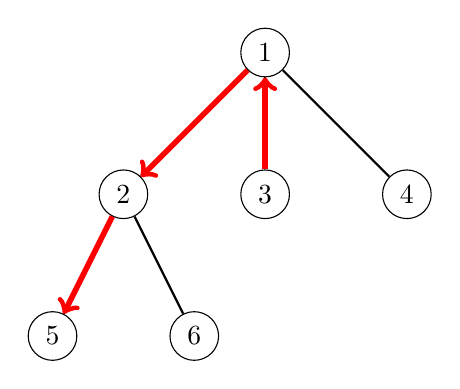
\begin{tikzpicture}[scale=0.9]
\node[draw, circle] (1) at (0,3) {$1$};
\node[draw, circle] (2) at (2,1) {$4$};
\node[draw, circle] (3) at (-2,1) {$2$};
\node[draw, circle] (4) at (0,1) {$3$};
\node[draw, circle] (6) at (-3,-1) {$5$};
\node[draw, circle] (7) at (-1,-1) {$6$};
\path[draw,thick,-] (1) -- (2);
\path[draw,thick,-] (1) -- (3);
\path[draw,thick,-] (1) -- (4);
\path[draw,thick,-] (3) -- (6);
\path[draw,thick,-] (3) -- (7);

\path[draw,thick,->,color=red,line width=2pt] (4) -- (1);
\path[draw,thick,->,color=red,line width=2pt] (1) -- (3);
\path[draw,thick,->,color=red,line width=2pt] (3) -- (6);
\end{tikzpicture}
\end{center}

Бір қарағанда $p$ төбесінен шығатын ең ұзын жолды таңдау керек сияқты көрінеді.
Бірақ ол әрқашан жұмыс жасамайды. Себебі $p$-төбенің ең ұзын
жолы $x$-төбеден өтуі мүмкін.
Төменде осы жағдайға мысал келтіреміз:
% At first glance, it seems that we should choose
% the longest path from $p$.
% However, this \emph{does not} always work,
% because the longest path from $p$
% may go through $x$.
% Here is an example of this situation:
\begin{center}
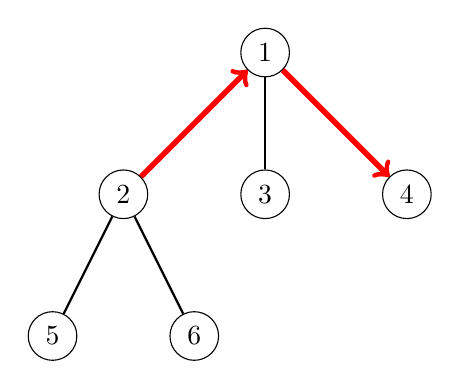
\begin{tikzpicture}[scale=0.9]
\node[draw, circle] (1) at (0,3) {$1$};
\node[draw, circle] (2) at (2,1) {$4$};
\node[draw, circle] (3) at (-2,1) {$2$};
\node[draw, circle] (4) at (0,1) {$3$};
\node[draw, circle] (6) at (-3,-1) {$5$};
\node[draw, circle] (7) at (-1,-1) {$6$};
\path[draw,thick,-] (1) -- (2);
\path[draw,thick,-] (1) -- (3);
\path[draw,thick,-] (1) -- (4);
\path[draw,thick,-] (3) -- (6);
\path[draw,thick,-] (3) -- (7);

\path[draw,thick,->,color=red,line width=2pt] (3) -- (1);
\path[draw,thick,->,color=red,line width=2pt] (1) -- (2);
\end{tikzpicture}
\end{center}

Десек те екінші бөлікті $O(n)$
уақытта шығара аламыз. Бұл ретте әр төбе үшін
екі максималды ұзындықты сақтау керек. Олар:
% Still, we can solve the second part in
% $O(n)$ time by storing \emph{two} maximum lengths
% for each node $x$:
\begin{itemize}
\item $\texttt{maxLength}_1(x)$:
$x$ төбесінен шығатын максималды ұзын жолдың мәні
\item $\texttt{maxLength}_2(x)$:
$x$ төбесінен шығатын бірінші бағыттан басқа максималды ұзын жолдың мәні
\end{itemize}
Мысалы, жоғарыдағы графта,
$\texttt{maxLength}_1(1)=2$ $1 \rightarrow 2 \rightarrow 5$ жолына сәйкес келсе,
ал $\texttt{maxLength}_2(1)=1$ $1 \rightarrow 3$ жолына сәйкес келеді.

Егер нәтижесінде $\texttt{maxLength}_1(p)$ мәніне 
сәйкес жол $x$ төбесінен өтсе, 
максималды ұзындық $\texttt{maxLength}_2(p)+1$-ге
тең болады. Басқа жағдайда $\texttt{maxLength}_1(p)+1$ 
мәніне тең болмақ.

\section{Бинарлы дарақ}

\index{бинарлы дарақ}

\begin{samepage}
Бинарлы дарақ -- әр төбенің 
сол және оң жақ ішдарақтары болатын түбірлі дарақ.
Төбенің сол немесе оң ішдарақтары болмауы да мүмкін. Осылайша
бинарлы дарақтағы әр төбенің нөл, бір немесе екі 
ұлы болады.
% A \key{binary tree} is a rooted tree
% where each node has a left and right subtree.
% It is possible that a subtree of a node is empty.
% Thus, every node in a binary tree has
% zero, one or two children.

Төмендегі дарақ бинарлы дараққа мысал бола алады:
\begin{center}
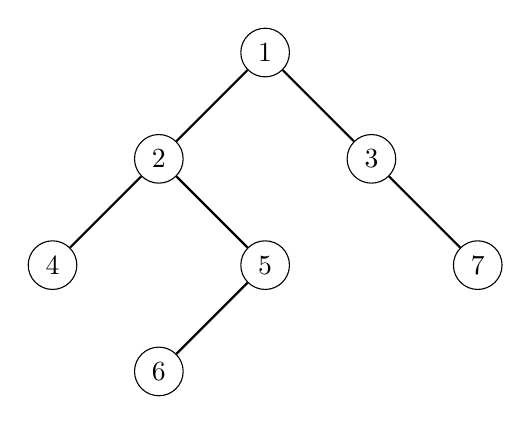
\begin{tikzpicture}[scale=0.9]
\node[draw, circle] (1) at (0,0) {$1$};
\node[draw, circle] (2) at (-1.5,-1.5) {$2$};
\node[draw, circle] (3) at (1.5,-1.5) {$3$};
\node[draw, circle] (4) at (-3,-3) {$4$};
\node[draw, circle] (5) at (0,-3) {$5$};
\node[draw, circle] (6) at (-1.5,-4.5) {$6$};
\node[draw, circle] (7) at (3,-3) {$7$};

\path[draw,thick,-] (1) -- (2);
\path[draw,thick,-] (1) -- (3);
\path[draw,thick,-] (2) -- (4);
\path[draw,thick,-] (2) -- (5);
\path[draw,thick,-] (5) -- (6);
\path[draw,thick,-] (3) -- (7);
\end{tikzpicture}
\end{center}
\end{samepage}

\index{кемімелі}
\index{бірізді}
\index{үдемелі}

Бинарлы дарақта төбелерді 
рекурсивті түрде үш түрлі әдіспен өтіп шығуға болады:

\begin{itemize}
\item \key{кемімелі} (pre-order): алдымен түбірден бастайды, сосын сол жақ ішдараққа 
өтіп, кейін оң жаққа барады.
% first process the root,
% then traverse the left subtree, then traverse the right subtree
\item \key{бірізді} (in-order): алдымен сол жақ ішдараққа барады, ал
содан кейін түбірге өтіп, соңында оң жақ ішдараққа жетеді.
% first traverse the left subtree,
% then process the root, then traverse the right subtree
\item \key{үдемелі} (post-order): алдымен сол жақ ішдараққа барады, ал содан соң
оң жақ ішдараққа өтіп, кейін түбірге келеді.
% first traverse the left subtree,
% then traverse the right subtree, then process the root
\end{itemize}

Берілген дарақтағы төбелердің тізімі кемімелі реттілік (pre-order) әдісімен
$[1,2,4,5,6,3,7]$ болса, бірізді реттілік (in-order) әдісінде 
$[4,2,6,5,1,3,7]$, ал үдемелі реттілік (post-order) әдісінде $[4,6,5,2,7,3,1]$
болады.
% For the above tree, the nodes in
% pre-order are
% $[1,2,4,5,6,3,7]$,
% in in-order $[4,2,6,5,1,3,7]$
% and in post-order $[4,6,5,2,7,3,1]$.

Егер біз дарақтың кемімелі (pre-order) және бірізді (in-order) реттіліктерінде өту
тізімін білсек, сол тізімге қарап
дарақты құрай аламыз.
Мысалы, егер кемімелі (pre-order) реттілікте өту тізімі $[1,2,4,5,6,3,7]$ және бірізді (in-order) реттілікте өту тізімі 
$[4,2,6,5,1,3,7]$ болса, жоғарыдағы дарақты құрауға болады.
Сондай-ақ үдемелі (post-order) және бірізді (in-order) реттілік тізімдері арқылы да ұқсас жолмен
дарақтың құрылымын табуға болады.

Бірақ дарақтың кемімелі (pre-order) және үдемелі (post-order) реттілік тізімдерін білсек,
жағдай басқаша болады.
Бұл жағдайда сәйкес келуі мүмкін дарақ құрылымдары көбейеді.
Мысалы, төмендегі дарақтарға қарайық:
\begin{center}
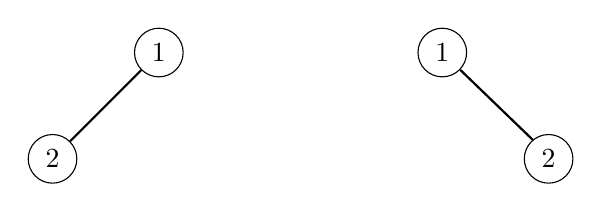
\begin{tikzpicture}[scale=0.9]
\node[draw, circle] (1) at (0,0) {$1$};
\node[draw, circle] (2) at (-1.5,-1.5) {$2$};
\path[draw,thick,-] (1) -- (2);

\node[draw, circle] (1b) at (0+4,0) {$1$};
\node[draw, circle] (2b) at (1.5+4,-1.5) {$2$};
\path[draw,thick,-] (1b) -- (2b);
\end{tikzpicture}
\end{center}
Екі дарақтың да кемімелі (pre-order) $[1,2]$ және үдемелі (post-order) $[2,1]$ реттілік тізімдері сәйкес.
Дегенмен дарақтардың құрылымдары әртүрлі.

